\chapter*{REMOTE ACCESS -TUTORIAL}
\section*{X2GO \& MobaXterm, Public Key Authentication and .bashrc Settings}
\subsection{X2Go Installation}
\begin{enumerate}
	\item
	X2Go is program used to run graphical applications on our Linux machines remotely. This uses a different technology from remote X, which results in better performance, especially when not on campus. This also allows for suspending and resuming sessions and programs, while they continue to run. This allows the use of long-running graphical applications.
	\item The X2Go Client software is already installed on all lab computers. For your personal computers, download the X2Go client for your operating system:
	\begin{enumerate}[label*=\arabic*.]
		\item macOS - 		\url{http://code.x2go.org/releases/X2GoClient_latest_macosx.dmg}
		\item Windows - \url{http://code.x2go.org/releases/X2GoClient_latest_mswin32-setup.exe}
	\end{enumerate}
	\item On macOS, mount the dmg file (your browser may do this for you after download) and drag the x2goclient application to your Applications folder. On Windows, double-click the downloaded setup file and follow the instructions in  wizard to install the software.
\end{enumerate}
\subsection{X2Go Configuration}
\begin{enumerate}[resume]
	\item When you first run the X2Go client, you will be presented with a "\emph{\textbf{New session}}" dialog. You should fill this in with this information:
	\item Session tab
	\begin{enumerate}[label*=\arabic*.]
		\item Session name - Any name you'd like to identify the session to yourself - if you're connecting to \emph{\textbf{i80labpc04.ira.uka.de}}, you might just want this to be " \emph{\textbf{i80labpc04}}" 
		\item Host - Full name of the server you're connecting to, e.g. 
		\emph{\textbf{i80labpc04.ira.uka.de}}
		\item All of our compute machines have the X2Go server installed
		\item Login -- Your user ID e.g. ``\emph{\textbf{asip04}}'' (be careful to use lower case)
		\item Session type - Select XFCE (this is the only supported session type) - see below for of session types.
	\end{enumerate}
\begin{figure}[!htb]
	\centering
	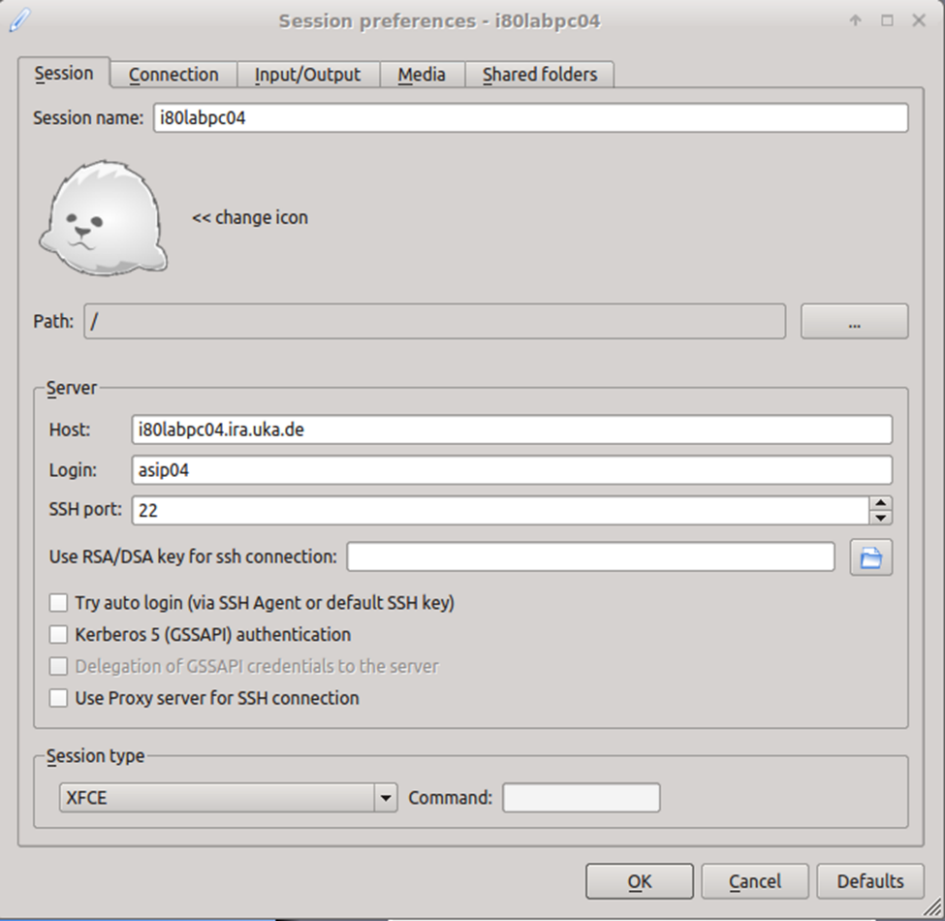
\includegraphics[width=0.5\textwidth]{src/images/image1.png}
	\caption{Session Tab}
	\label{fig:fig1}
\end{figure}
	\item Connection tab
	\begin{enumerate}[label*=\arabic*.]
		\item Connection speed - Set the connection speed you will most often use for this connection 
		\item The default ADSL is fine for most connections, but if you are on campus, you will get better graphics performance if you choose LAN
	\end{enumerate}
\begin{figure}[!htb]
	\centering
	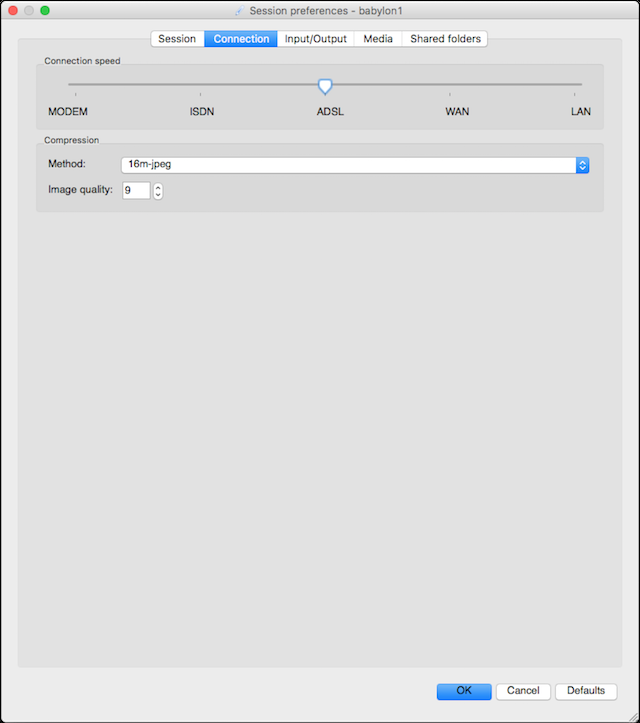
\includegraphics[width=0.5\textwidth]{src/images/image2.png}
	\caption{Connection Tab}
	\label{fig:fig2}
\end{figure}
	\item Input/output tab
	\begin{enumerate}[label*=\arabic*.]
		\item Display - select whether you want to run full screen or at a specific resolution
	\end{enumerate}
	\item  Media
	\begin{enumerate}[label*=\arabic*.]
		\item Client side printing support - be sure to uncheck this box or you may get errors when starting the session
	\end{enumerate}
\end{enumerate}
\begin{figure}[!htb]
	\centering
	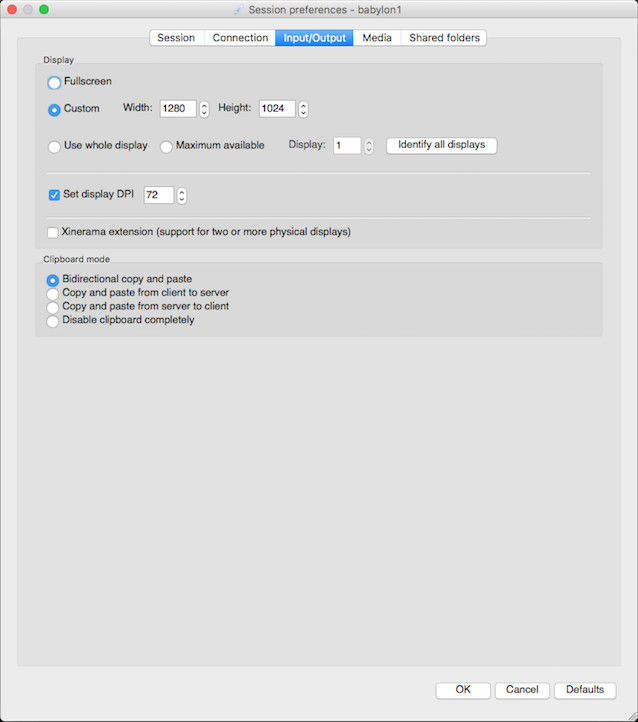
\includegraphics[width=0.5\textwidth]{src/images/image3.png}
	\caption{Input/output Tab}
	\label{fig:fig3}
\end{figure}

\begin{figure}[!htb]
	\centering
	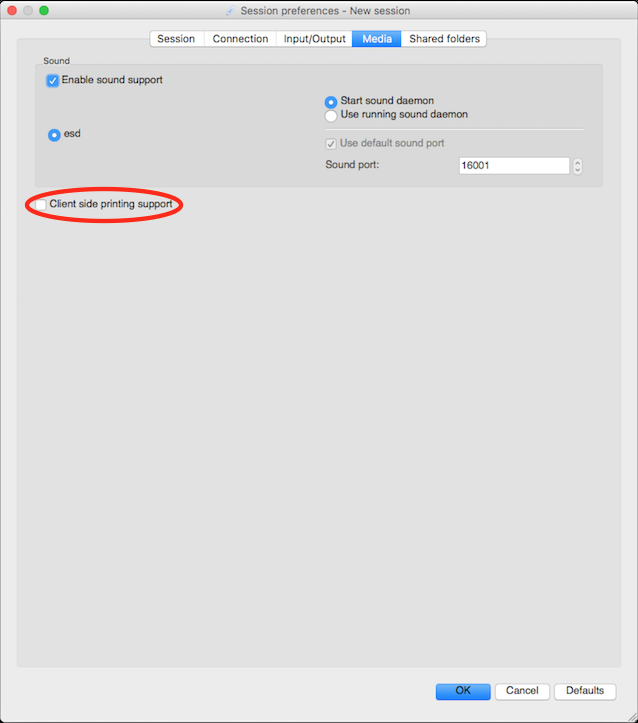
\includegraphics[width=0.6\textwidth]{src/images/image4.png}
	\caption{Media Tab}
	\label{fig:fig4}
\end{figure}

\begin{figure}[!htb]
	\centering
	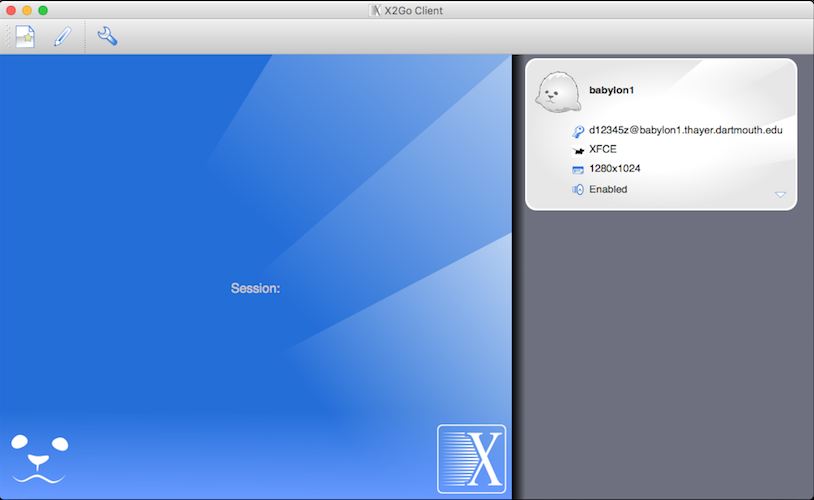
\includegraphics[width=0.6\textwidth]{src/images/image5.png}
	\caption{Main Client Screen}
	\label{fig:fig5}
\end{figure}
\subsection{X2Go Session Types}
\begin{enumerate}[resume]
	\item The session types that we support are:
	\begin{enumerate}[label*=\arabic*.]
		\item XFCE (recommended) - This is a low-power window manager that is the only one supported in the current version of Ubuntu
		\item Published applications - This allows you to run one or more applications directly, rather than a full desktop session. See below for how to run published applications
	\end{enumerate}
\end{enumerate}
\subsection{X2Go Connecting}
\begin{enumerate}[resume]
	\item To start the session, click on it and provide your password where prompted
\begin{figure}[!htb]
	\centering
	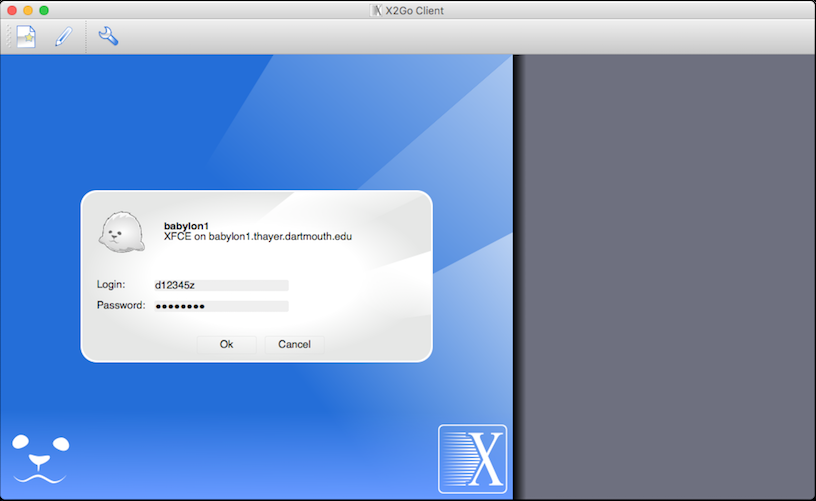
\includegraphics[width=0.6\textwidth]{src/images/image6.png}
	\caption{Login Screen}
	\label{fig:fig6}
\end{figure}
	\item After you click OK, it will connect to the server and start your session. Watch the Status line to see what's happening. Once the status is "running," your session should launch.
	\item When you first connect to a particular server, you may get a dialog box asking you to accept the host key. Click Yes to accept it:
\begin{figure}[!htb]
	\centering
	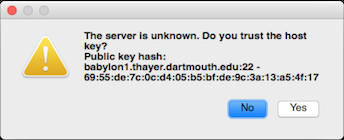
\includegraphics[width=0.6\textwidth]{src/images/image7.png}
	\caption{Host Key Authentication}
	\label{fig:fig7}
\end{figure}
	\item To suspend a session, click the suspend button:
\begin{figure}[!htb]
	\centering
	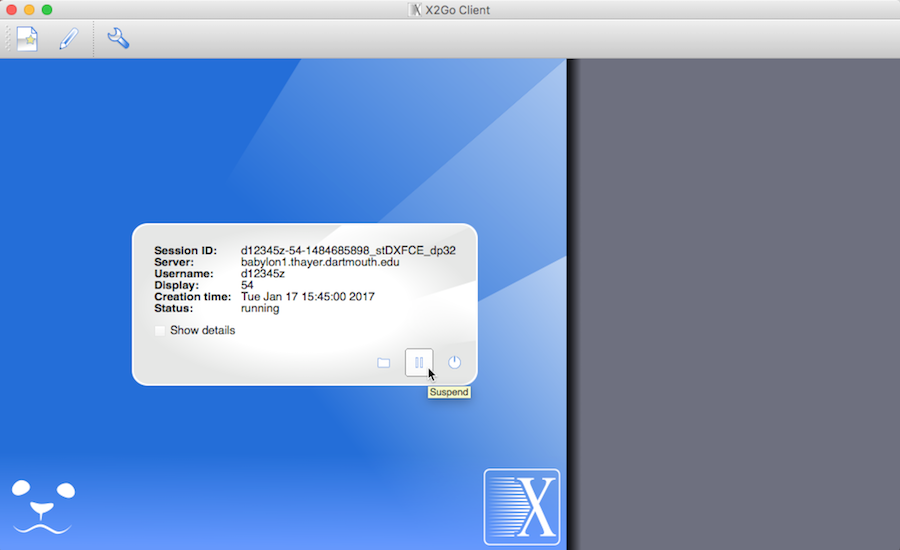
\includegraphics[width=0.6\textwidth]{src/images/image8.png}
	\caption{Suspending a Session}
	\label{fig:fig8}
\end{figure}
	\item To terminate, either log out of your session or click the terminate button:
\begin{figure}[!htb]
	\centering
	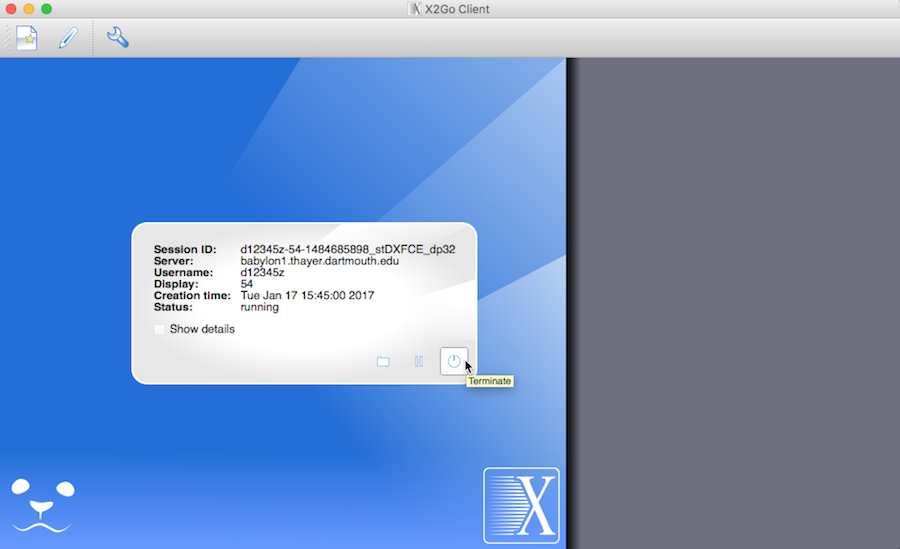
\includegraphics[width=0.6\textwidth]{src/images/image9.png}
	\caption{Terminating a Session}
	\label{fig:fig9}
\end{figure}
\end{enumerate}
\subsection{X2Go Resuming}
\begin{enumerate}[resume]
	\item If you have a single session open on a particular server and you reconnect with the same client, it will automatically re-connect to your session.
	\item If you are connecting from a different client or have multiple sessions on the same server, you'll be presented a list to either resume an existing session or create a new one:
\begin{figure}[!htb]
	\centering
	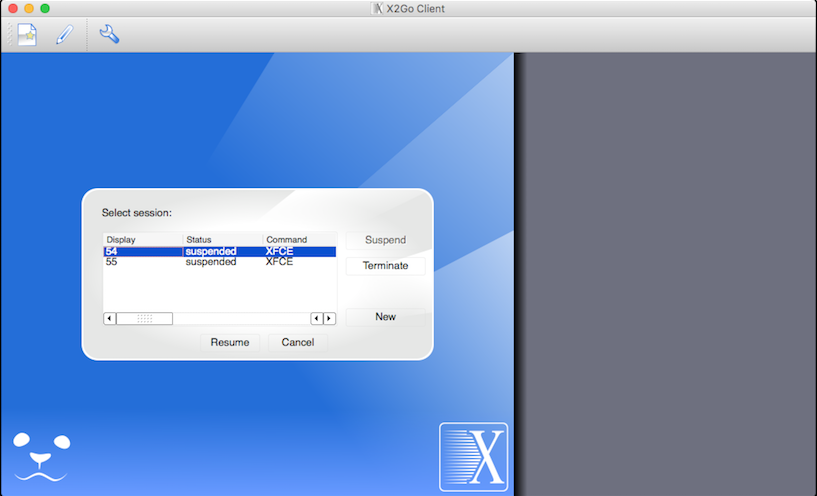
\includegraphics[width=0.6\textwidth]{src/images/image10.png}
	\caption{Resuming a Session}
	\label{fig:fig10}
\end{figure}
\end{enumerate}
\subsection{X2Go Published Applications}
\begin{enumerate}[resume]
	\item If you choose the "Published Applications" session, after you connect the Status will change to running, but it will appear that nothing has happened. To choose an application, click the "Applications" button: 
\begin{figure}[!htb]
	\centering
	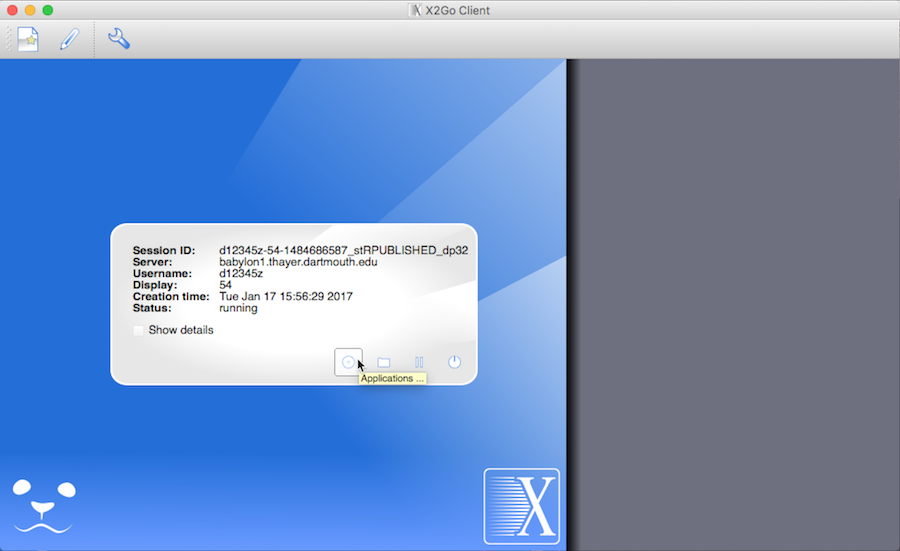
\includegraphics[width=0.6\textwidth]{src/images/image11.png}
	\caption{Published Applications}
	\label{fig:fig11}
\end{figure}
	\item This will then bring up a dialog from which you can choose an application to run. All Thayer-specific applications are interspersed under the "Other" section:
\begin{figure}[!htb]
	\centering
	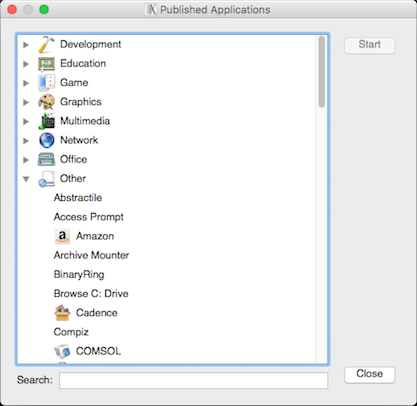
\includegraphics[width=0.6\textwidth]{src/images/image12.png}
	\caption{Applications}
	\label{fig:fig12}
\end{figure}
	\item When you click "Start," be patient. This dialog does not go away and some programs may take several seconds to start up. Clicking Start more than once will launch multiple instances of the same app. 
	\item Fonts for Windows
	\item When using the X2Go client on Windows, there may be some older programs (e.g. Cadence) where fonts do not show up properly. Symptoms you may see are either blocky, illegible fonts or instances where fonts disappear because they are white on a white background. If you experience any of these, you can install a font package that should eliminate most of these issues. Keep in mind that this is only needed if you are running the X2Go client on Windows.
	\item First, if you haven't already, follow the instructions at Thayer Shares Connecting to connect to Thayer Shares. Navigate to the Courses share (P:), and go to the software\textbackslash x2go folder. In this folder, double-click the vcxsrv\_fonts.exe file to install the fonts. Depending on your security settings, you may need to drag this file to your local computer before double-clicking on it.
	\item Other Settings
	\item If you are using a Mac and need to use the Alt key within remote sessions, you need to change the X11 preferences. Run XQuartz directly from within Applications-\textgreater Utilities. Then, select the X11-\textgreater Preferences... menu item, select the Input tab, and check the box next to "Option keys send Alt\_L and Alt\_R." Close the preferences window and quit X11. Then, restart X2Go and when you log into a remote session, the option key (also labeled alt on most Mac keyboards) will send the Alt key to the remote side.
\begin{figure}[!htb]
	\centering
	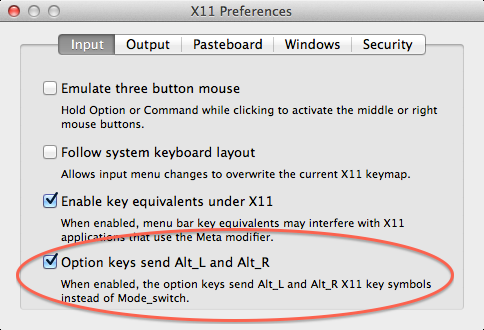
\includegraphics[width=0.6\textwidth]{src/images/image13.png}
	\caption{X11 Preferences}
	\label{fig:fig13}
\end{figure}
\end{enumerate}

\textbf{\hfill\break
}
\section*{MobaXterm CLIENT -TUTORIAL}
\subsection{MobaXterm Installation}
\begin{enumerate}
	\item Download MobaXterm from \url{https://mobaxterm.mobatek.net/download.html}
	\item Install it with default settings.
\end{enumerate}
\subsection{MobaXterm Configuration}
\begin{enumerate}[resume]
	\item Click on "Sessions" and then on "SSH".
\begin{figure}[!htb]
	\centering
	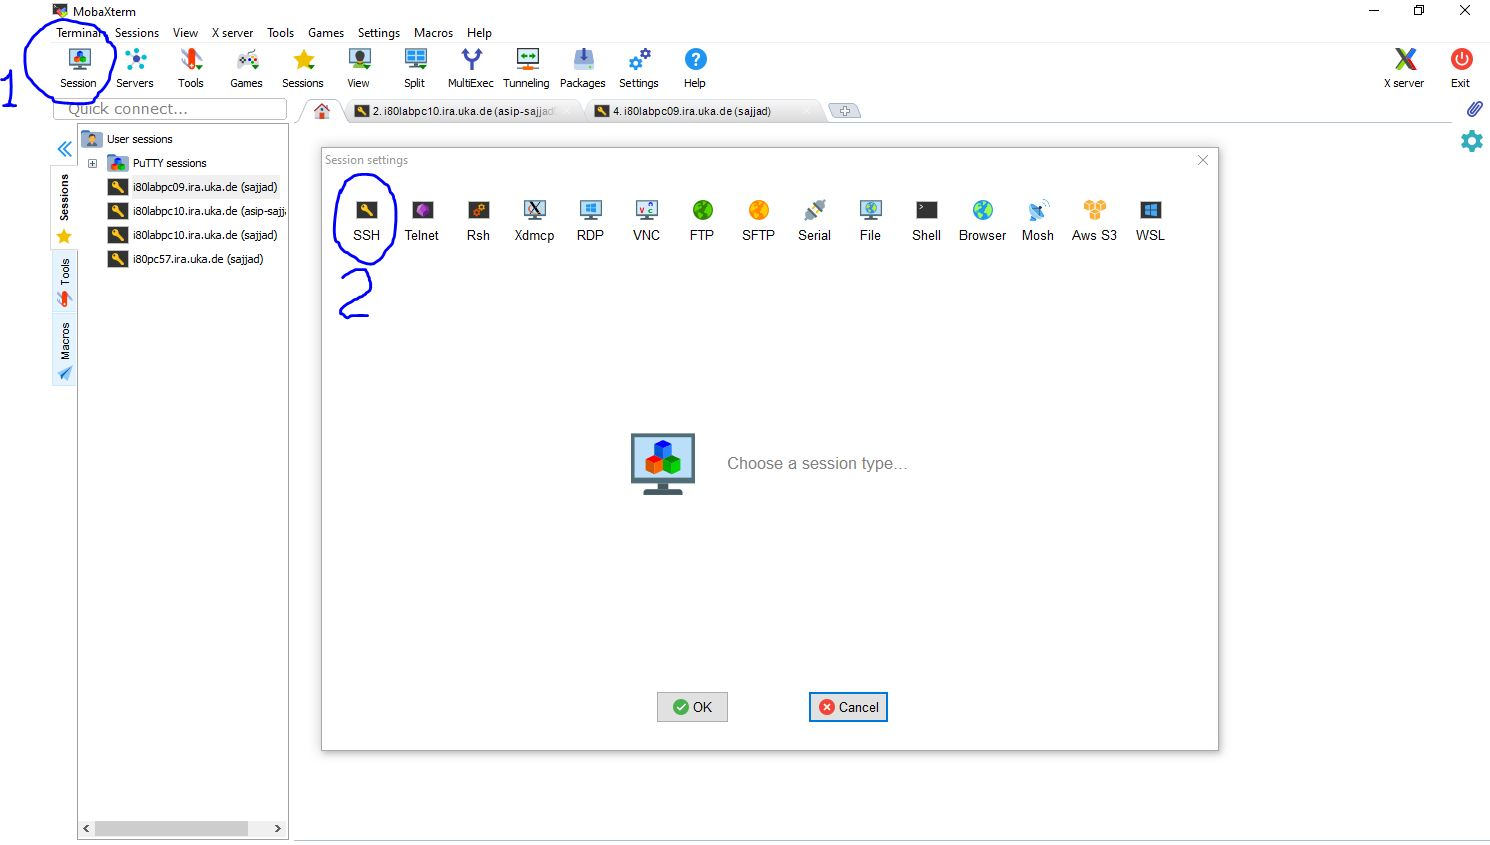
\includegraphics[width=0.6\textwidth]{src/images/image14.JPG}
	\caption{SSH Session}
	\label{fig:fig14}
\end{figure}
	\item In the new windows "Session settings", enter \textbf{Remote host} as ``\emph{i80labpcXX.ira.uka.de}'', tick the box "\textbf{Specify user name}" and then enter your user name as ``\emph{asip-abcdnn}''.
\begin{figure}[!htb]
	\centering
	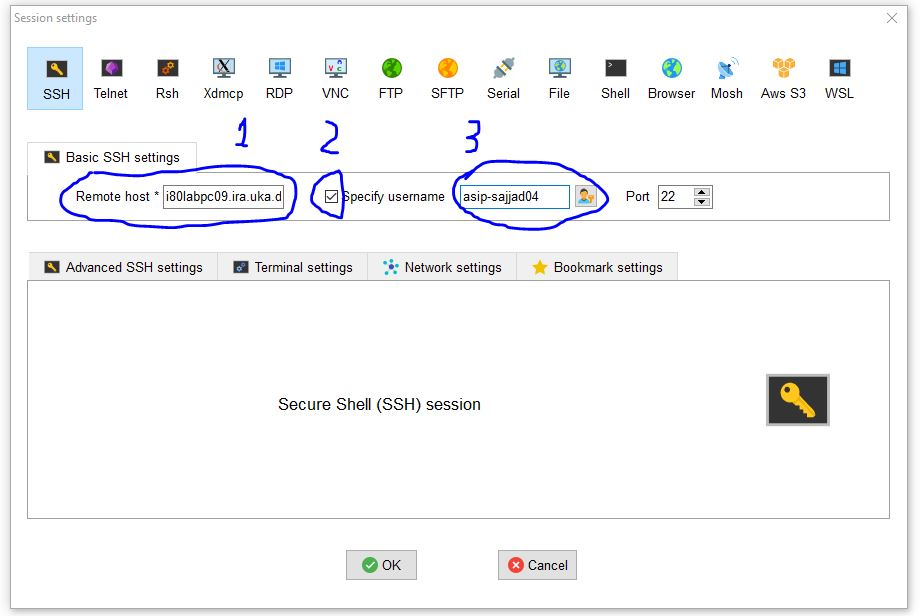
\includegraphics[width=0.6\textwidth]{src/images/image15.JPG}
	\caption{Session Settings}
	\label{fig:fig15}
\end{figure}
	\item Press OK. It will ask for the user password.
	\item Enter your password and press Enter.
\begin{figure}[!htb]
	\centering
	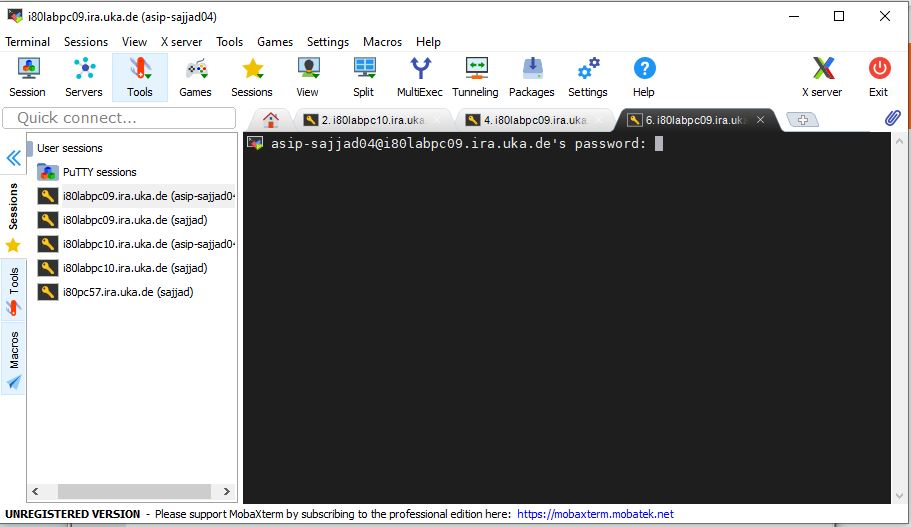
\includegraphics[width=0.6\textwidth]{src/images/image16.JPG}
	\caption{Logging in and Requiring Password}
	\label{fig:fig16}
\end{figure}
	\item You are now logged into the lab PC using MobaXterm.
\begin{figure}[!htb]
	\centering
	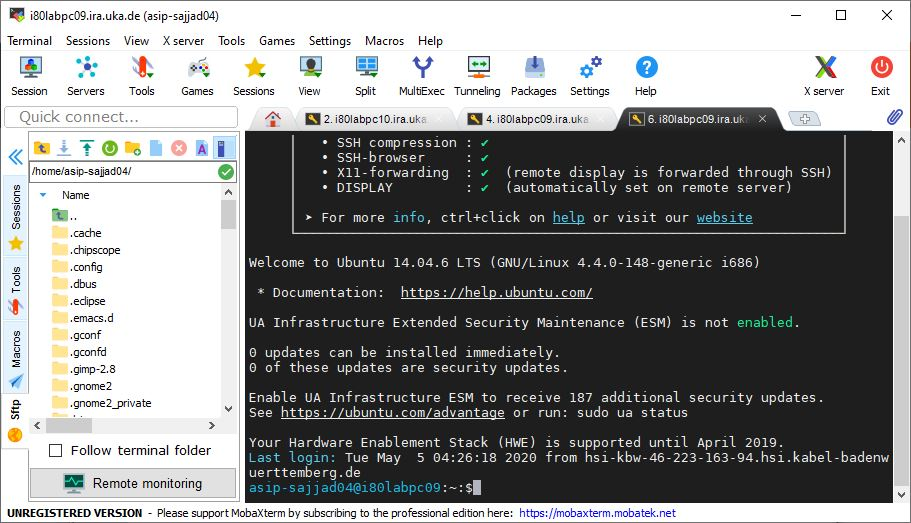
\includegraphics[width=0.6\textwidth]{src/images/image17.JPG}
	\caption{Logged into Remote PC}
	\label{fig:fig17}
\end{figure}
\end{enumerate}
\subsection{Recommended Practice.}
\begin{enumerate}[resume]
\item It is \textbf{recommended} to log into \textbf{i80pc57} as this PC contains the ASIPmeister software. Try to perform lab on this PC. Use \textbf{i80labpc10} when you need to implement your applications on FPGA.
\item To repeatedly login to some PC and avoid password, use DSA-keys and copy to desired PC.
\item Type "\textbf{ssh-keygen -t dsa}" and press Enter. Leave the default options. Leave the password empty.
\begin{lstlisting}
asip-sajjad04@i80labpc09:~:$ssh-keygen -t dsa
Generating public/private dsa key pair.
Enter file in which to save the key (/home/asip-sajjad04/.ssh/id_dsa):
/home/asip-sajjad04/.ssh/id_dsa already exists.
Overwrite (y/n)? y
Enter passphrase (empty for no passphrase):
Enter same passphrase again:
Your identification has been saved in /home/asip-sajjad04/.ssh/id_dsa.
Your public key has been saved in /home/asip-sajjad04/.ssh/id_dsa.pub.
The key fingerprint is:
af:c3:84:62:4e:f4:e6:5e:cb:d1:03:19:ff:63:a9:ad asip-sajjad04@i80labpc09
The key's randomart image is:
+--[ DSA 1024]----+
|                 |
|                 |
|        .        |
|    .    +       |
|   . . .S .      |
|    + + .+ . .   |
|   + + oo + =    |
|    . .oo+ = .   |
|     .. +.E..    |
+-----------------+
\end{lstlisting}
\item Then copy this generated DSA-key to desired PC by type following command and enter your password.
\begin{lstlisting}
asip-sajjad04@i80labpc09:~:$ssh-copy-id -i ~/.ssh/id_dsa.pub asip-sajjad04@i80pc57
/usr/bin/ssh-copy-id: INFO: attempting to log in with the new key(s), to filter out any that are already installed
/usr/bin/ssh-copy-id: INFO: 1 key(s) remain to be installed -- if you are prompted now it is to install the new keys
asip-sajjad04@i80pc57's password:

Number of key(s) added: 1

Now try logging into the machine, with:   "ssh 'asip-sajjad04@i80pc57'"
and check to make sure that only the key(s) you wanted were added.
\end{lstlisting}
\item Now log into i80pc57 using ``ssh -X'' it will ask for the password.
\begin{lstlisting}[language=bash]
asip-sajjad04@i80labpc09:~:$ssh -X i80pc57
Last login: Wed May  6 05:11:07 2020 from i80labpc09.irf.uni-karlsruhe.de
asip-sajjad04@i80pc57:~:$
\end{lstlisting}
\end{enumerate}
\subsection{Setting up .bashrc.user}
\begin{enumerate}[resume]
\item Whenever you are logged into any PC, this file is executed at the login. Please set different variables in this file carefully. Usually the following variables should be like this:
\begin{lstlisting}[language=bash]
asip-sajjad04@i80pc57:~:$cat .bashrc.user
export ASIPS_LICENSE=29000@i80asip.ira.uka.de
export PATH=/AM/ASIPmeister/bin:$PATH
export ASIP_APDEV_SRCROOT=/home/asip00/epp/AM_tools
export PATH=/usr/java/jre1.6.0_45/bin:$PATH
export ASIPmeister_Home=/AM/ASIPmeister
export ASIPmeister_HOME=/AM/ASIPmeister
. /home/adm/modelsim_66d.setup
. /home/adm/xilinx_13.2_32bit.setup
asip-sajjad04@i80pc57:~:$
\end{lstlisting}
\end{enumerate}